\documentclass[aspectratio=43]{beamer}
\usepackage[utf8]{inputenc}
\usepackage{multicol}
\usepackage{fontspec}
\setsansfont{Songti SC} % font name is case-sensitive

\title{密文重复数据删除机制的\\频率分析攻击}
\date{\today}
\author[Tinoryj]{任彦璟}

\usetheme{material}

\useLightTheme
\usePrimaryBlue
\useAccentOrange

\begin{document}

\begin{frame}
\titlepage
\end{frame}

\begin{frame}
\begin{card}
现有频率分析攻击在加密重复数据删除中效果不佳,\\[2mm]如何有针对性的提高攻击效果?
\end{card}
\end{frame}


\begin{frame}{目录}
\begin{card}
\tableofcontents
\end{card}
\end{frame}

\section{对选题的分析}

\begin{frame}{对选题的分析}
\begin{card}
\begin{itemize}
    \item 背景知识
    \item 两大核心问题
    \item 研究的意义
    \item 研究的目的
\end{itemize}
\end{card}
\end{frame}

\begin{frame}{背景知识-重复数据删除}
\centering
\cardImg{img/DedupSystemStorageMode}{\textwidth}
\begin{card}
重复数据删除系统的存储方式
\end{card}   
\end{frame}

\begin{frame}{背景知识-重复数据删除}
\centering
\cardImg{img/DedupSystemView}{\textwidth}
\begin{card}
重复数据删除系统的运作流程
\end{card}   
\end{frame}

\begin{frame}{背景知识-密文重复数据删除}
\centering
\cardImg{img/EncryptDedupSystemLogic}{\textwidth}
\begin{card}
密文重复数据删除的运作流程
\end{card}   
\end{frame}

\begin{frame}{背景知识-频率分析攻击}
\begin{card}
频率分析是一种针对确定性加密的密码分析技术,被应用\\[2mm]于破解匿名查询日志、破坏关键词隐私、重构密文数据库\\[2mm]记录等实际攻击。
\end{card}   
\end{frame}

\begin{frame}{背景知识-MLE加密}
\begin{card}
消息锁定加密确立了加密重复数据删除的密码学基础:基\\[2mm]于数据内容产生密钥,从而将相同明文加密为相同密文。
\end{card}   
\end{frame}

\begin{frame}{两大核心问题}
\begin{card}
数据块频率泄漏问题:加密重复数据删除广泛应用MLE,\\[2mm]导致数据块的频率信息泄漏。
\end{card}
\begin{card}
针对数据块的频率分析攻击,与现有攻击目标(查询日志\\[2mm]条目、关键词、数据库记录等)相比,数据块数量极其庞\\[2mm]大(呈千万级),并且大量数据块具有相同频率,致使当\\[2mm]前的频率分析攻击算法难以适用。
\end{card}
\end{frame}

\begin{frame}{研究的意义}
\begin{card}
填补频率分析攻击研究空白。
\end{card}
\begin{card}
对理解加密重复数据删除的实际安全性,并降低其在非适\\[2mm]合场景下的误用风险具有重要作用。
\end{card}
\end{frame}


\begin{frame}{研究的目的}
\begin{card}
在理论上:构造针对加密重复数据删除的频率分析攻击,\\[2mm]揭示实践中的安全隐患。
\end{card}
\begin{card}
在技术上:以理论研究为支撑,设计并实现针对加密重复\\[2mm]数据删除的频率分析攻击工具,并在真实系统中进行理论\\[2mm]验证和攻击效果测试。 
\end{card}
\end{frame}

\section{国内外研究现状}

\begin{frame}{国内外研究现状}
\begin{card}
\begin{itemize}
    \item 加密重复数据删除
    \item 频率分析攻击
    \item 密文重复数据删除的其他攻击
\end{itemize}
\end{card}
\end{frame}

\begin{frame}{加密重复数据删除}
\begin{card}
密码学理论基础:\textbf{消息锁定加密(MLE)}
\end{card}

\begin{itemize}
    \item 收敛加密(CE)使用明文的哈希值作为MLE密钥,并基于\\[2mm]密文哈希值计算指纹,以识别重复数据。
    \item 哈希收敛加密(HCE)与CE具有相同的MLE密钥产生规则\\[2mm],但基于明文哈希值计算指纹。
    \item 随机收敛加密(RCE)使用随机密钥加密以产生非确定的密\\[2mm]文,同时基于明文哈希值来进行重复检查。
    \item 收敛扩散(CD)使用明文哈希值作为秘密共享的输入种子\\[2mm],提高了密文存储的可靠性。
\end{itemize}

\end{frame}

\begin{frame}{频率分析攻击}
\begin{card}
针对确定性加密的密码分析技术。
\end{card}
\begin{card}
面向加密重复数据删除,已有工作提出了基于数据块局部\\[2mm]性(chunk locality)的频率分析攻击。
\end{card}
\end{frame}

\begin{frame}{密文重复数据删除的其他攻击}
\begin{card}
加密重复数据删除可能遭受边信道攻击、副本伪造攻击、\\[2mm]
基于数据块长度的攻击等威胁,但这些攻击可通过所有权\\[2mm]
证明、守卫解密(guarded decryption)、固定长度分块等措\\[2mm]施进行防御。
\end{card}
\begin{card}
本研究的频率分析攻击超出了现有保护措施的防御范畴。
\end{card}
\end{frame}

\section{主要研究内容}

\begin{frame}{对选题的分析}
\begin{card}
\begin{itemize}
    \item 三个主要研究内容
    \item 研究的技术路线
\end{itemize}
\end{card}
\end{frame}

\begin{frame}{三个主要研究内容}
\begin{card}
研究基于数据特征的新型频率分析攻击技术,提高传统频\\[2mm]率分析的攻击效果。
\end{card}
\begin{card}
分别从抵抗频率排序干扰和降低攻击发生条件两方面改进\\[2mm]攻击技术。
\end{card}
\begin{card}
实现针对真实系统的频率分析攻击原型,并分析该攻击对\\[2mm]各类数据安全性的影响。
\end{card}
\end{frame}

\begin{frame}{研究的技术路线}
\centering
\cardImg{img/TechnicalRoute}{\textwidth}
\begin{card}
本研究的技术路线
\end{card}   
\end{frame}


\section{攻击方案的设计}

\begin{frame}{攻击方案的设计}
\begin{card}
\begin{itemize}
    \item 已有工作:基于数据块局部性的攻击
    \item 本课题研究内容:基于分布的攻击
    \item 本课题研究内容:基于聚类的攻击
\end{itemize}
\end{card}
\end{frame}

\begin{frame}{基于数据块局部性的攻击}
\centering
\cardImg{img/BaseFrequencyAttack}{\textwidth}
\begin{card}
已有工作提出的基于数据块局部性的攻击方案
\end{card}   
\end{frame}

\begin{frame}{基于分布的攻击}
\centering
\cardImg{img/DistributionAttack}{\textwidth}
\begin{card}
设计的基于分布的攻击的攻击方案
\end{card}   
\end{frame}

\begin{frame}{基于聚类的攻击}
\centering
\cardImg{img/ClusteringAttack}{\textwidth}
\begin{card}
设计的基于聚类的攻击方案
\end{card}   
\end{frame}

\section{研究结果与分析}

\begin{frame}{研究结果与分析}
\begin{card}
\begin{itemize}
    \item 基于分布的攻击-部分结果
    \item 基于聚类的攻击-部分结果
\end{itemize}
\end{card}
\end{frame}

\begin{frame}{基于分布的攻击结果}
\begin{figure}[!htbp]
    \centering
    \begin{tabular}{p{.48\linewidth}p{.48\linewidth}}
        \multicolumn{2}{c}{
\includegraphics[width=.35\textwidth]{img/legend-effectiveness.pdf}}  \\
        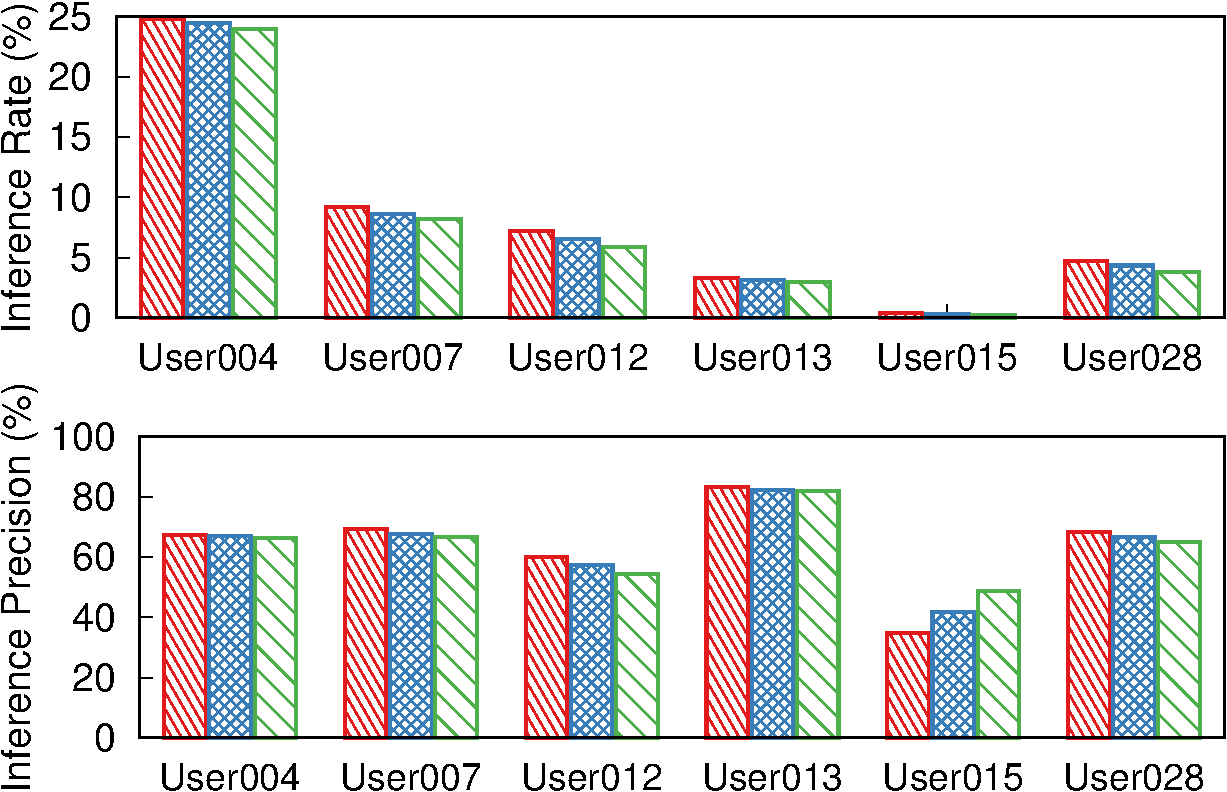
\includegraphics[width=\linewidth]{img/distribution-effectiveness-wo-size.pdf} &
        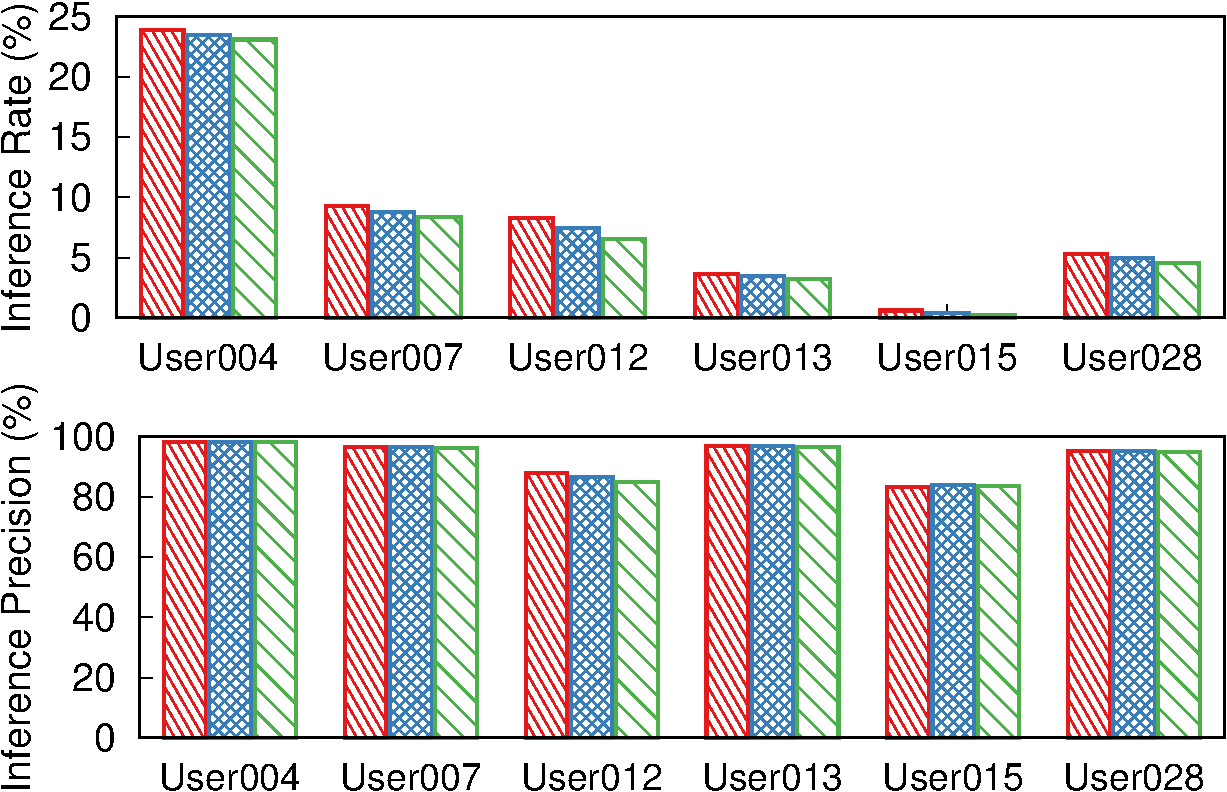
\includegraphics[width=\linewidth]{img/distribution-effectiveness-w-size.pdf}\\
    \end{tabular}
\end{figure}
\begin{card}
设计的基于分布的攻击方案在FSL数据集中的攻击效果\\[2mm](左无数据块大小信息辅助,右有数据块大小信息辅助)
\end{card}  
\end{frame}

\begin{frame}{基于聚类的攻击结果}
\begin{figure}[!htbp]
    \centering
    \begin{tabular}{p{.48\linewidth}p{.48\linewidth}}
        \multicolumn{2}{c}{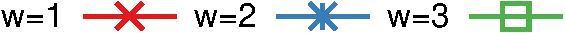
\includegraphics[width=.35\textwidth]{img/clu-effect-bar.pdf}}  \\
        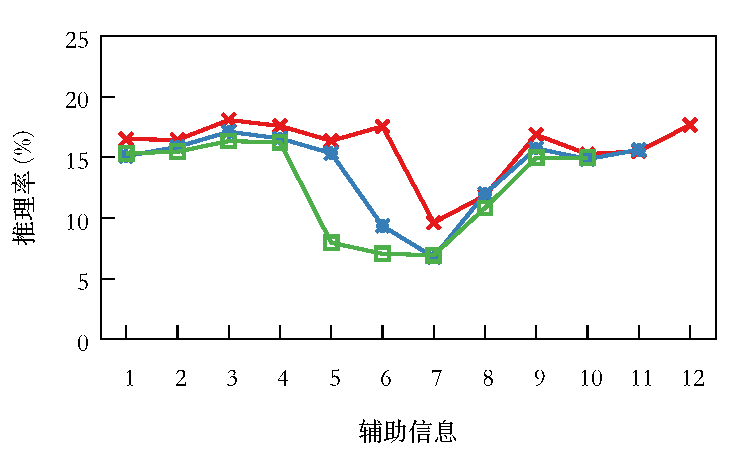
\includegraphics[width=\linewidth]{img/clu-effect-rate.pdf} &
        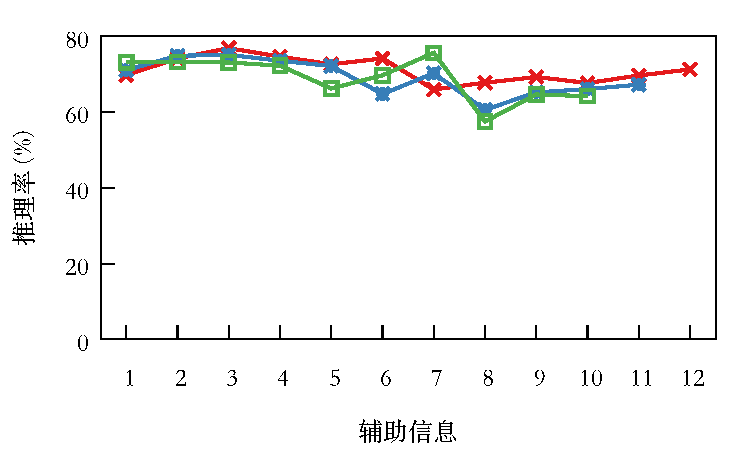
\includegraphics[width=\linewidth]{img/clu-effect-pre.pdf}\\
    \end{tabular}
\end{figure}
\begin{card}
设计的基于聚类的攻击方案在VM数据集中的攻击效果。
\end{card}  
\end{frame}

\section{总结建议与参考文献}
\begin{frame}{总结建议与参考文献}
\begin{card}
\begin{itemize}
    \item 关于研究的总结
    \item 针对本文提出的攻击的建议
    \item 参考文献
\end{itemize}
\end{card}
\end{frame}

\begin{frame}{关于研究的总结}
\begin{card}
加密重复数据删除应用确定性加密,并由此泄漏了明文的\\[2mm]
频率。研究重新审视了频率分析引起的安全漏洞,并证明\\[2mm]
加密重复数据删除更容易受到推理攻击。
\end{card}

\begin{card}
研究提出了两种新的频率分析攻击方法,它们在攻击者所\\[2mm]
具有的条件的不同假设下都能实现高推理率和高推理精度。
\end{card}
\end{frame}

\begin{frame}{关于研究的总结}
\begin{card}
利用三个真实世界的数据集来验证评估这两种攻击方法,\\[2mm]
提出关于其性质的各种新观察,并进一步分析它们如何带
来实际性的损害。
\end{card}
\begin{card}
研究还讨论了加密重复数据删除应对频率分析攻击的可能\\[2mm]
的对策及其相应的优缺点,以建议从业者安全地实现和部\\[2mm]
署加密重复数据删除存储系统。
\end{card}
\end{frame}

\begin{frame}{针对本文提出的攻击的建议}
\begin{card}
\begin{itemize}
    \item \textbf{防止频率泄漏}:MinHash加密、加入冗余数据块。
    \item \textbf{防止顺序泄漏}:添加扰动。
    \item \textbf{防止大小泄漏}:数据填充、固定大小分块。
\end{itemize}
\end{card}
\end{frame}

\begin{frame}{参考文献}
...
\end{frame}

%
%\begin{frame}{Setup}
%\begin{card}
%Setup is really easy: 
%{\color{primary}\textbackslash usetheme\{material\}}
%\end{card}
%\begin{card}
%Further you might want to customize the background with: \\[2mm]
%{\color{primary}\textbackslash useLightTheme} or {\color{primary}\textbackslash useDarkTheme} \\[2mm]
%and primary and accent colors.
%\end{card}
%\end{frame}
%
%\begin{frame}{Setup -- colors}
%\begin{card}
%There are some colors from the Material Design guidelines coded in. You access those by: \\[2mm]
%{\color{primary} \textbackslash usePrimary[Color]} and {\color{primary}\textbackslash useAccent[Color]}\\[2mm]
%{\tiny {\color{primary}Color} $\in \{$ Red, Pink, Purple, Deep Purple, Indigo, Blue, Light Blue, Cyan, Teal, Green, Light Green, Lime, Yellow, Amber, Orange, Deep Orange, Brown, Grey, Blue Grey $\}$} \\[2mm]
%or you can pick your own:\\[2mm]
%{\color{primary} \textbackslash usePrimary\{primary color, darker primary color, text color\}}
%{\color{primary} \textbackslash useAccent\{primary color, text color\}}\\[2mm]
%{\color{primary} darker primary color} is just darker version of {\color{primary} primary color} and {\color{primary} text color} is color of text on {\color{primary} primary} or {\color{primary} accent colors}.
%\end{card}
%\end{frame}
%
%\begin{frame}{Card}
%\begin{card}
%All content should only appear in cards. There are several variants:
%\begin{itemize}
%\item plain card
%\item card with a title
%\item card with an image
%\item tiny card
%\end{itemize}
%\end{card}
%\end{frame}
%
%\begin{frame}{plain card}
%\begin{card}
%\end{card}
%
%\begin{card}
%{\color{primary} \textbackslash begin\{card\}\\[2mm]}
%\null\qquad \textit{[your content here]}\\[2mm]
%{\color{primary} \textbackslash end\{card\}}
%\end{card}
%\end{frame}
%
%\begin{frame}{card with a title}
%\begin{card}[Title]
%\end{card}
%
%\begin{card}
%{\color{primary} \textbackslash begin\{card\}[Title]\\[2mm]}
%\null\qquad \textit{[your content here]}\\[2mm]
%{\color{primary} \textbackslash end\{card\}}
%\end{card}
%\end{frame}
%
%\begin{frame}{card with an image}
%\centering
%\cardImg{img/rudolfinum.jpg}{0.5\textwidth}
%
%\begin{card}
%{\color{primary} \textbackslash cardImg\{file name\}\{width\}}
%\end{card}
%\end{frame}
%
%\begin{frame}{tiny card}
%\begin{cardTiny}
%\end{cardTiny}
%
%\begin{card}
%{\color{primary} \textbackslash begin\{cardTiny\}\\[2mm]}
%\null\qquad \textit{[your content here]}\\[2mm]
%{\color{primary} \textbackslash end\{cardTiny\}}
%\end{card}
%\begin{card}
%Tiny card is useful for labels where too much whitespace gets in the way. 
%\end{card}
%\end{frame}
%
%\begin{frame}{Cards can be filled with anything you want}
%
%\begin{card}
%\centering$V(x) = \left\{ y \in \mathbb{R}^n \,|\, \forall z \in P, z\neq x:\, \|y-x\|\leq\|y-z\| \right\}$
%\end{card}
%
%\begin{card}
%\centering
%\begin{tabular}{lcr}
%left & center & right \\
%\hline
%1 & 2 & 3 \\
%\end{tabular}
%\end{card}
%
%\begin{card}
%\begin{theorem}[Pythagorean]
%The sum of the areas of the two squares on the legs equals the area of the square on the hypotenuse.
%\end{theorem}
%\end{card}
%\end{frame}
%
%\begin{frameImg}{img/rudolfinum.jpg}
%\vspace*{60mm}
%\begin{cardTiny}
%Lastly it is possible to set image as a background for a frame:\\[2mm]
%{\color{primary} \textbackslash begin\{frameImg\}["height"]\{file name\}\\[2mm]}
%\null\qquad \textit{[your content here]}\\[2mm]
%{\color{primary} \textbackslash end\{frameImg\}}
%\end{cardTiny}
%\end{frameImg}
%
%\begin{frameImg}[height]{img/rudolfinum.jpg}
%\vspace*{60mm}
%\begin{cardTiny}
%Parameter {\color{primary} ["height"]} determines the dimension that is stretched to cover the frame ({\color{primary} ["width"]} is default).
%\end{cardTiny}
%\end{frameImg}
%
%\begin{frame}
%\begin{multicols}{2}
%[
%\begin{cardTiny}
%Two images side by side with columns.
%\end{cardTiny}
%]
%\centering
%\cardImg{img/rudolfinum.jpg}{0.48\textwidth}
%
%\cardImg{img/rudolfinum.jpg}{0.48\textwidth}
%\end{multicols}
%\end{frame}
%
%\begin{frame}
%\begin{card}
%That is all for now. Despite having successfully presented several project with this theme, it is still work in progress. If this manual is not clear enough, you can also review it's source, that may bring more clarity.
%\end{card}
%\begin{card}
%Feel free to submit any issues you find on github: \\
%{\footnotesize \url{https://github.com/edasubert/beamerMaterialDesign}}
%\end{card}
%\begin{card}
%This theme is released under MIT license. Feel free to modify or improve or whatever. 
%\end{card}
%\end{frame}

\end{document}
